% ==============================================================================
\section{Integración de los módulos de representación}
\label{sec:dev_integracion}
% ==============================================================================

Los tres módulos anteriores trabajan en secuencia dentro del ciclo principal del
sistema. El mismo ciclo corre en el programa de la Raspberry Pi del prototipo
(\texttt{main\_pi.py}, sin interfaz gráfica), en el programa de pruebas para la
computadora portátil (\texttt{main\_lap.py}, con interfaz gráfica y entrada de cámara,
video o simulación) y en el procesamiento de videos (\texttt{video\_a\_mapa.py}). El
Algoritmo~\ref{alg:dev_representacion} resume el orden de las operaciones y sustituye
al pseudocódigo integrado de representación que se planteó en TT1
(Apéndice~\ref{apend:representa}).

\begin{center}
\captionof{algorithm}{Ciclo integrado de los módulos de representación}
\label{alg:dev_representacion}
\end{center}
\vspace{-1.8cm}
\rule{\textwidth}{0.4pt}
\vspace{-0.9cm}
\begin{algorithmic}[1]

\Statex \textbf{INICIO:}
\State mapa $\gets$ abrir\_mapa\_por\_bloques(carpeta) \Comment{crea o restaura los bloques}
\State slam $\gets$ EKF en (0, 0, 0)
\State slam.cargar\_referencias(mapa.referencias\_guardadas) \Comment{re-localización}

\Statex
\Statex \textbf{CICLO (por cada cuadro de la cámara):}
\State movimiento, cabeceo $\gets$ odometría.actualizar(cuadro) \Comment{IMU o flujo óptico}
\State detecciones $\gets$ visión.procesar(cuadro, giro = movimiento.$\Delta\theta$)
\If{toca segmentación (cada N cuadros)}
    \State peligros $\gets$ detector\_peligros.procesar(cuadro)
\EndIf
\State lecturas $\gets$ ultrasónicos.leer()
\State lecturas $\gets$ validar\_con\_ultrasonido(detecciones, lecturas, cabeceo)
\State observaciones $\gets$ fusionar(detecciones + peligros, lecturas)
\State salida $\gets$ slam.ciclo(movimiento, observaciones)
\State pose $\gets$ (salida.x, salida.y, salida.$\theta$)
\State mapa.actualizar\_con\_rayos(pose, slam.observaciones\_para\_mapa() + rayos\_sin\_eco(lecturas))
\State mapa.despejar\_huella(pose)
\State eventos $\gets$ mapa.actualizar\_posición(pose, slam.referencias)
\State cuadro\_nav $\gets$ construir\_cuadro\_navegación(slam, mapa, detecciones, lecturas)
\State entregar cuadro\_nav y eventos a navegación, alertas e interacción

\Statex
\Statex \textbf{AL TERMINAR:}
\State mapa.guardar\_todo();\; mapa.guardar\_referencias(slam.exportar\_referencias())

\end{algorithmic}
\vspace{-0.9cm}
\rule{\textwidth}{0.4pt}

\subsection{Funcionamiento con video}

Las Figuras~\ref{fig:cap_oficina_1} a \ref{fig:cap_oficina_3} son capturas de la
interfaz de \texttt{main\_lap.py} mientras procesa el recorrido de una oficina grabado
con un teléfono. A la izquierda de cada captura está la imagen de la cámara con las
detecciones; en verde los objetos estáticos y en rojo los marcados como móviles, junto
con su clase, el estado de las puertas y la distancia estimada. A la derecha está el
mapa global por bloques, con los \emph{landmarks} etiquetados, la pose del usuario
(punto rojo con su orientación) y su elipse de incertidumbre. Abajo aparece la barra
de navegación con la distancia libre y el riesgo de cada sector, y la alerta del
momento.

\begin{figure}[H]
    \centering
    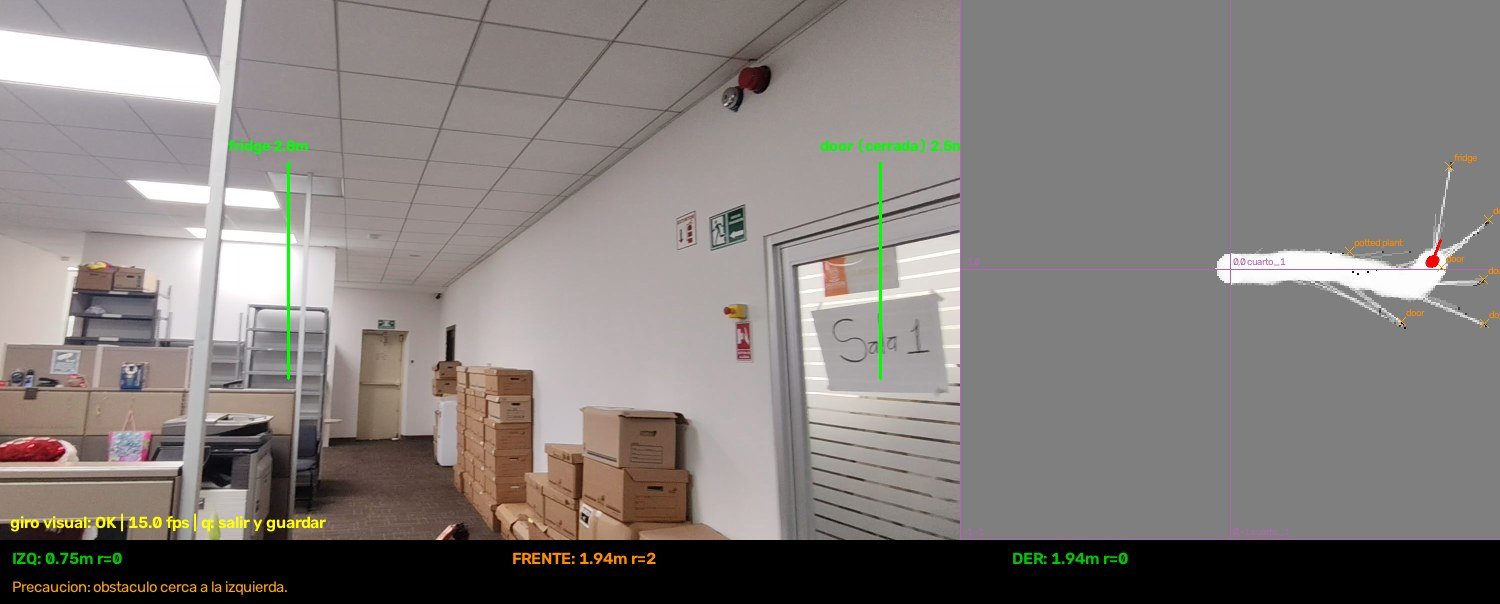
\includegraphics[width=\textwidth]{Capturas_TT2/cap_oficina_f241.jpg}
    \caption{Inicio del recorrido. Se detectan una puerta cerrada a 2.5~m y un
    refrigerador, el mapa empieza a registrar la franja recorrida y la barra avisa de un
    obstáculo a 0.75~m a la izquierda.}
    \label{fig:cap_oficina_1}
\end{figure}

\begin{figure}[H]
    \centering
    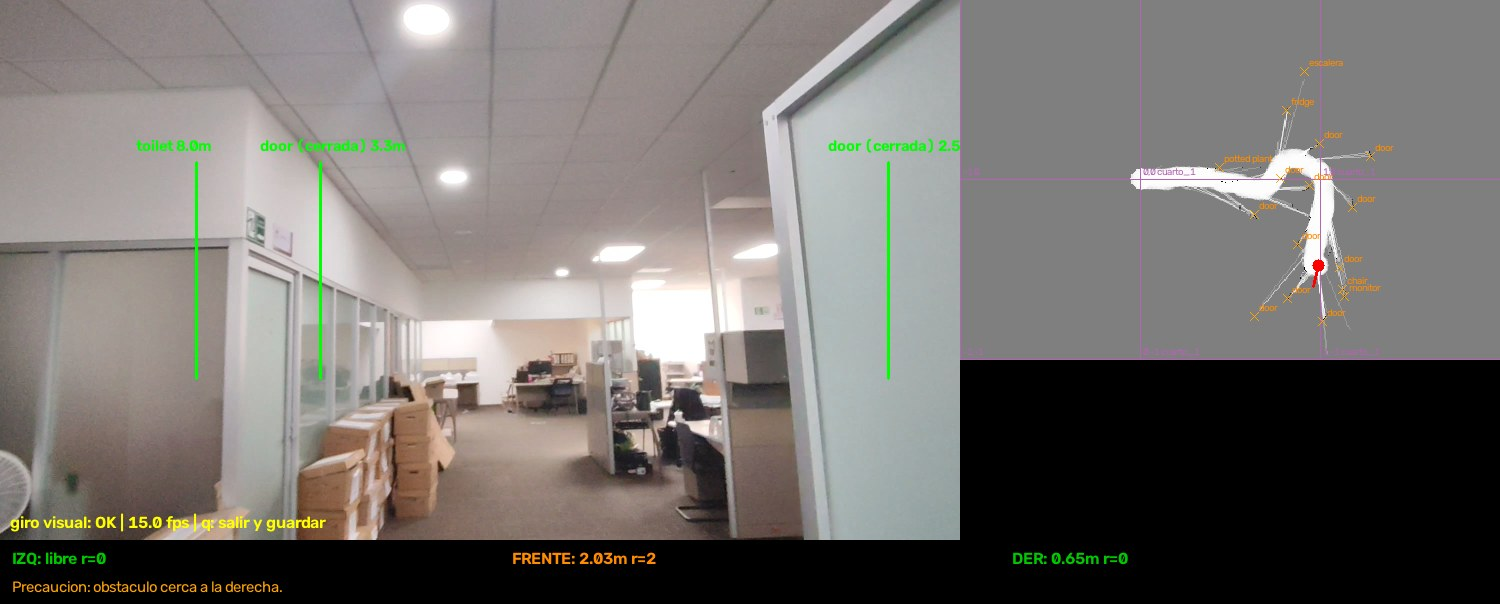
\includegraphics[width=\textwidth]{Capturas_TT2/cap_oficina_f481.jpg}
    \caption{Al girar hacia el pasillo, el SLAM ya mantiene varias puertas como
    \emph{landmarks} y el mapa muestra el cambio de dirección.}
    \label{fig:cap_oficina_2}
\end{figure}

\begin{figure}[H]
    \centering
    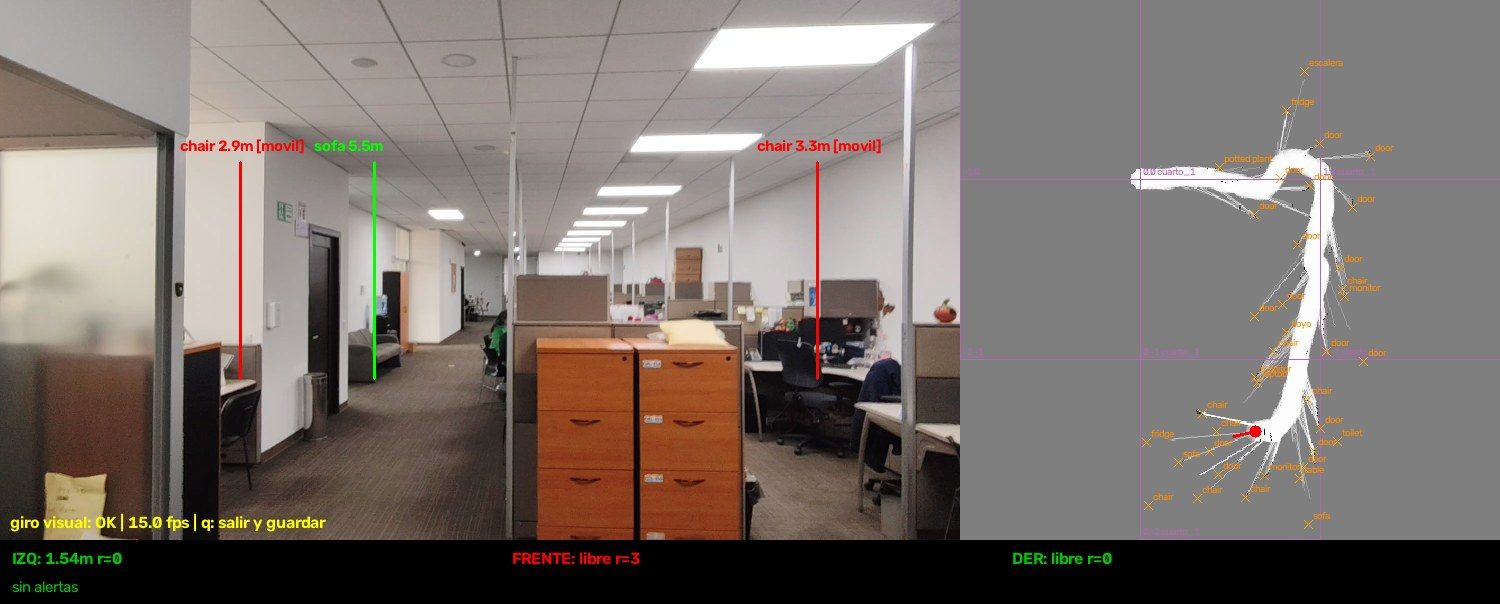
\includegraphics[width=\textwidth]{Capturas_TT2/cap_oficina_f901.jpg}
    \caption{Final del recorrido, con siete bloques y 39 \emph{landmarks} confirmados.
    Dos sillas aparecen como móviles por un error del rastreador al avanzar el
    usuario.}
    \label{fig:cap_oficina_3}
\end{figure}

En las capturas se ven también errores de la percepción que llegan a la
representación. En la Figura~\ref{fig:cap_oficina_2} aparece un inodoro a 8~m que no
existe, y en la Figura~\ref{fig:cap_oficina_3} dos sillas que no se mueven se marcan como
móviles, porque el rastreador compensa el giro del usuario pero no su avance. Las reglas
del SLAM contienen el daño, ya que los objetos móviles no se usan como \emph{landmarks}
y los falsos positivos aislados no llegan a los avistamientos necesarios para
confirmarse.

\subsection{Funcionamiento en el prototipo}

\TODO{capturas o registros de \texttt{main\_pi.py} durante un recorrido con el
prototipo: mapa resultante, \emph{landmarks}, alertas emitidas y comentarios del
recorrido}.

\subsection{Tiempos de procesamiento}

La Tabla~\ref{tab:tiempos_ciclo} desglosa el tiempo promedio por ciclo. La columna de
la computadora portátil se midió al procesar el video de la oficina (456 cuadros, uno de
cada dos del video original) con todos los modelos en CPU; la de la Raspberry Pi
corresponde al prototipo en operación.

\begin{table}[H]
\centering
\caption{Tiempo promedio por ciclo}
\label{tab:tiempos_ciclo}
\renewcommand{\arraystretch}{1.2}
\begin{tabular}{|p{7.4cm}|c|c|}
\hline
\textbf{Etapa} & \textbf{Apple M4 (ms)} & \textbf{Raspberry Pi (ms)} \\
\hline
Estimación de giro y caminata por flujo óptico & 5.4 & \TODO{} \\
Detección de objetos (YOLOv8s-seg) & 92.4 & \TODO{} \\
Segmentación de peligros y puertas (SegFormer, amortizado) & 77.5 & \TODO{} \\
\hline
SLAM (EKF, asociación y gestión de \emph{landmarks}) & 0.27 & \TODO{} \\
Ray Casting y actualización del mapa por bloques & 0.23 & \TODO{} \\
Construcción del cuadro de navegación & 0.51 & \TODO{} \\
\hline
\textbf{Subtotal de los módulos de representación} & \textbf{1.01} & \TODO{} \\
\hline
\end{tabular}
\end{table}

Los módulos de representación se llevan alrededor de un milisegundo por ciclo en la
computadora portátil, menos del 1\,\% del tiempo total. Por sí solos podrían correr a
cientos de hertz, muy por encima de los 10~Hz que pide RNF-03; el cuello de botella es la
percepción visual. Por eso el SLAM y el mapa siguen actualizándose con la odometría en
los ciclos en que la visión no entrega resultados, y la segmentación solo se ejecuta cada
cierto número de cuadros. En la Raspberry Pi el ciclo completo corre a \TODO{frecuencia
del ciclo completo en la Raspberry Pi}.

\subsection{Cumplimiento de requerimientos}

La Tabla~\ref{tab:req_representacion} relaciona los requerimientos de los módulos de
representación con su estado.

\begin{longtable}{|p{1.6cm}|p{4.2cm}|p{2.4cm}|p{6.2cm}|}
\caption{Estado de los requerimientos de los módulos de representación}
\label{tab:req_representacion} \\
\hline
\textbf{Req.} & \textbf{Descripción breve} & \textbf{Estado} & \textbf{Evidencia} \\
\hline
\endfirsthead
\hline
\textbf{Req.} & \textbf{Descripción breve} & \textbf{Estado} & \textbf{Evidencia} \\
\hline
\endhead
RF-14 & Estimación continua de la pose & Cumplido & EKF con ATE de 0.21~m en
simulación y error acotado con odometría sesgada (Tabla~\ref{tab:slam_deriva}). \\
\hline
RF-15 & Mapa incremental sin mapa previo & Cumplido &
Figura~\ref{fig:mapeo_evolucion} y mapas de 19 videos reales. \\
\hline
RF-16 & Zonas libres y ocupadas & Cumplido & Mapa log-odds con tres estados, capa de
peligros y mapa local de dos canales. \\
\hline
RF-17 & Actualización dinámica & Cumplido & Los obstáculos nuevos aparecen en el mapa;
los que desaparecen se liberan con ecos precisos y los falsos peligros de piso, con los
rayos de piso libre (Secciones~\ref{sec:dev_ray} y \ref{sec:dev_mapeo}). \\
\hline
RNF-03 & Mapa a 10~Hz o más & \TODO{} & 1~ms por ciclo en la computadora portátil
(Tabla~\ref{tab:tiempos_ciclo}); \TODO{frecuencia en la Raspberry Pi}. \\
\hline
RNF-05 & Hardware limitado & \TODO{} & Estado de pose de tamaño fijo y memoria acotada a
25 bloques (unos 3~MB); \TODO{uso de memoria y CPU en la Raspberry Pi}. \\
\hline
RNF-09 & Comportamiento conservador & Cumplido & Confianza que baja sin correcciones
(Figura~\ref{fig:slam_incertidumbre}) y distancia mínima por sector. \\
\hline
RNF-13 & Operación sin internet & Cumplido & Ningún módulo de representación necesita
conexión y los mapas se guardan localmente. \\
\hline
RNF-14 & Modularidad & Cumplido & Comunicación solo por las estructuras de
\texttt{interfaces.py}; el mismo código trabaja con cámara, video y simulación. \\
\hline
\end{longtable}
